%%%%%%%%%%%%%%%%%%%%%%%%%%%%%%%%%
%% INSTALACION LINUX
%%%%%%%%%%%%%%%%%%%%%%%%%%%%%%%%%
\subsection{Instalación en Linux}
Para la instalación de Docker CE en los sistemas operativos GNU/Linux se tienen diferentes métodos como la instalación de los repositorios, descargar los ejecutables para la distribución específica o la ejecución de un script que contiene los pasos de instalación básica, la ejecución del script se realiza con los siguientes comandos, y su salida se puede observar en la figura \ref{fig:InstalacionDockerLinux1}

\begin{figure}[!hbtp]
	\centering
	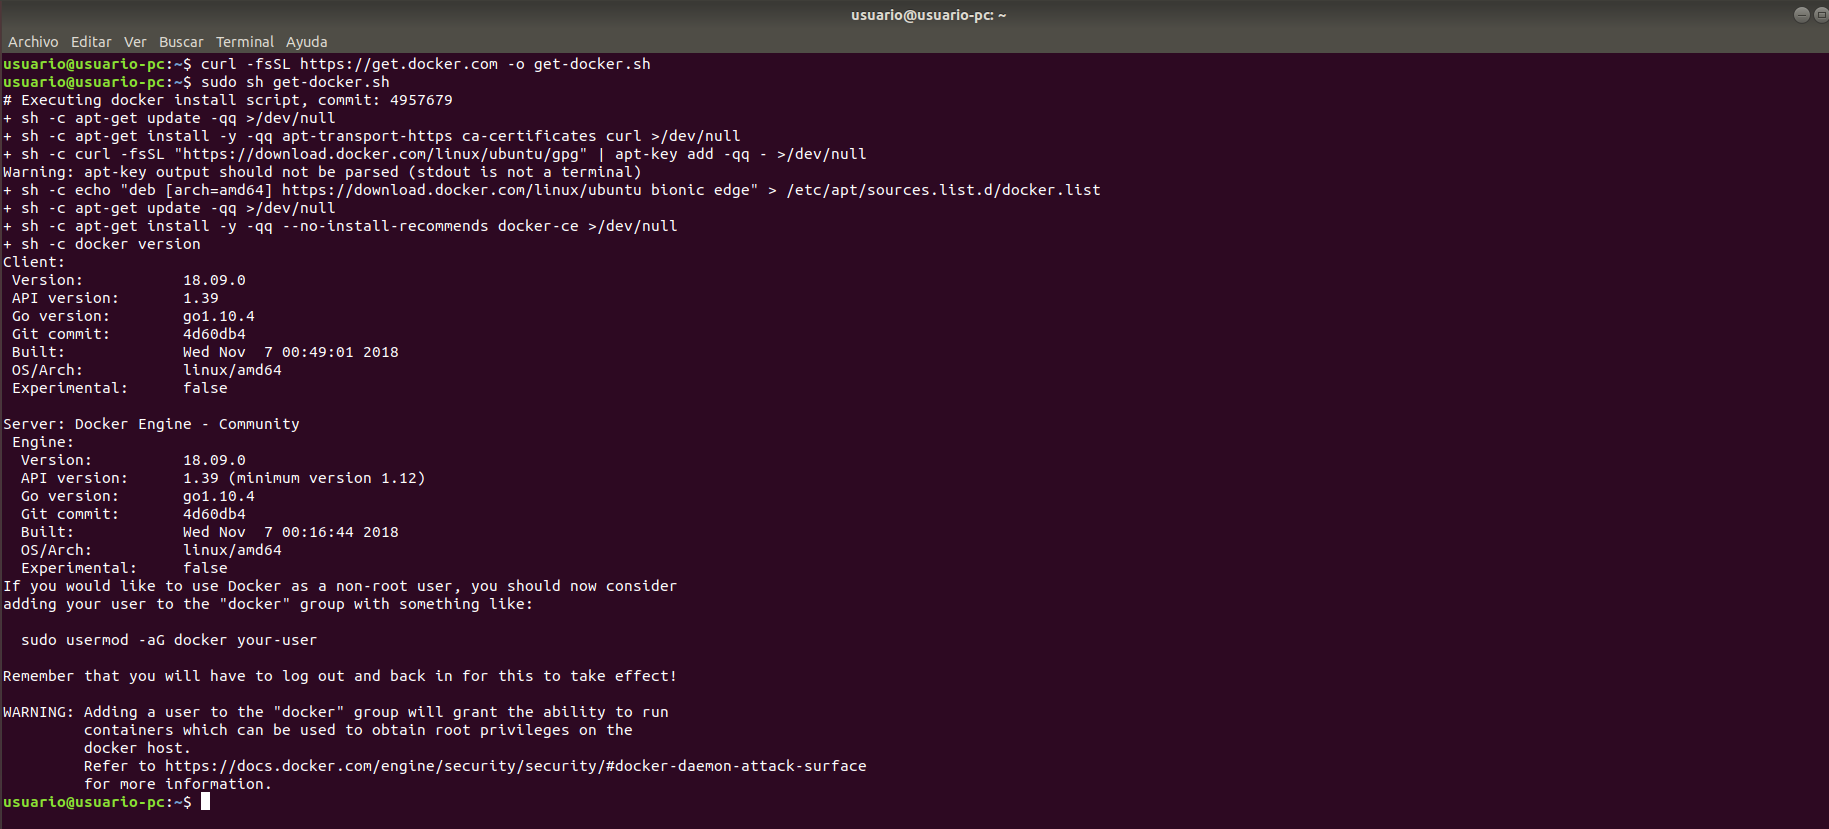
\includegraphics[width=\linewidth]{RE05_Docker/Instalacion_Linux/REDocker_Instalacion_Linux.png}
	\vspace{-0.2cm}
	\caption{Salida del script de instalación Docker }
	\label{fig:InstalacionDockerLinux1}
\end{figure}

Al terminar la instalación de Docker CE se puede verificar la versión básica de Docker con el comando \begin{commandshell}{docker version}\end{commandshell}
en la figura \ref{fig:InstalacionDockerLinux2} se puede ver la salida del comando.

\begin{figure}[!hbtp]
	\centering
	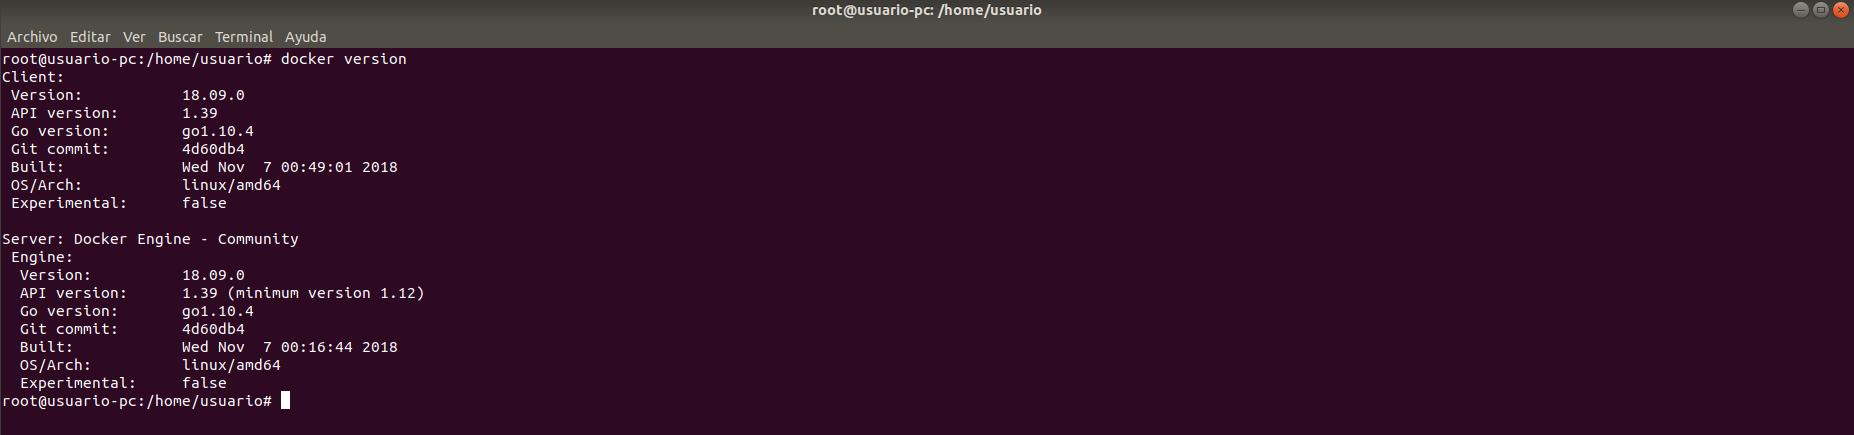
\includegraphics[width=\linewidth]{RE05_Docker/Instalacion_Linux/REDocker_Instalacion_Linux2.png}
	\vspace{-0.2cm}
	\caption{Salida del comando docker version }
	\label{fig:InstalacionDockerLinux2}
\end{figure}
%%%%%%%%%%%%%%%%%%%%%%%%%%%%%%%%%
%% INSTALACION Windows
%%%%%%%%%%%%%%%%%%%%%%%%%%%%%%%%%
\subsection{Instalación Microsoft Windows}
Para poder realizar la instalación de Docker en microsoft windows de una forma nativa, sólo funcionará con las versiones Microsoft Windows 10 Professional y Microsoft Windows 10 Enterprise, en las figuras \ref{fig:InstalacionDockerWin1},\ref{fig:InstalacionDockerWin2},\ref{fig:InstalacionDockerWin3},\ref{fig:InstalacionDockerWin4} se muestra la interacción con el asistente de instalación de Docker.

\begin{figure}[!hbtp]
	\centering
	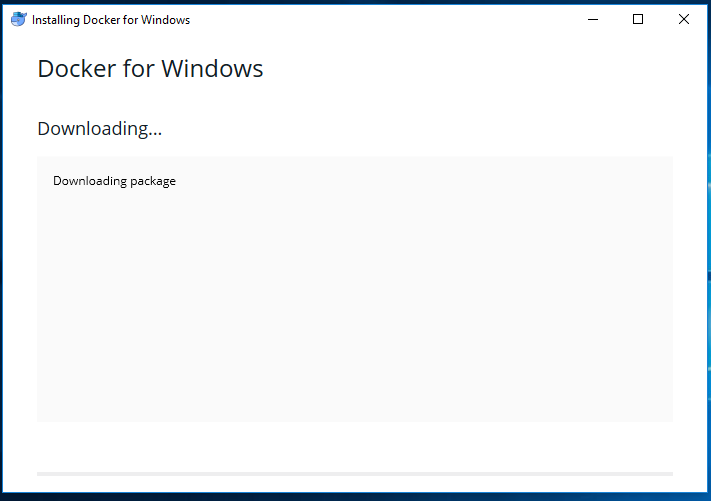
\includegraphics[width=\linewidth]{RE05_Docker/Instalacion_Windows/REDocker_Instalacion_Windows01.png}
	\vspace{-0.2cm}
	\caption{Asistente instalación Docker: Descarga paquetes necesarios}
	\label{fig:InstalacionDockerWin1}
\end{figure}

\begin{figure}[!hbtp]
	\centering
	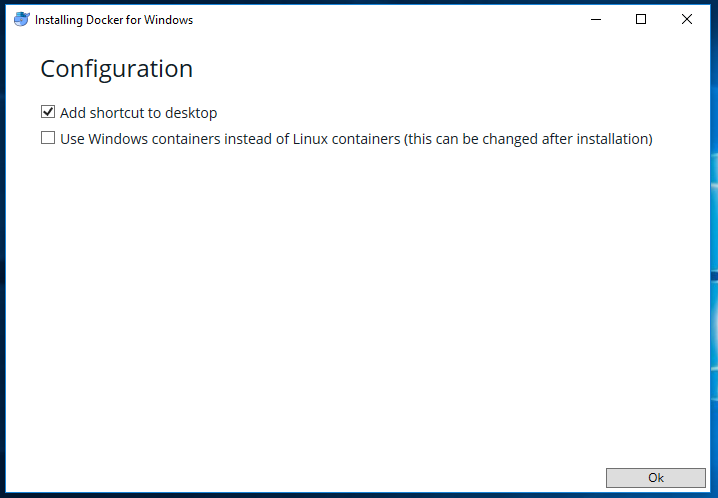
\includegraphics[width=\linewidth]{RE05_Docker/Instalacion_Windows/REDocker_Instalacion_Windows02.png}
	\vspace{-0.2cm}
	\caption{Asistente instalación Docker: Configuración básica}
	\label{fig:InstalacionDockerWin2}
\end{figure}

\begin{figure}[!hbtp]
	\centering
	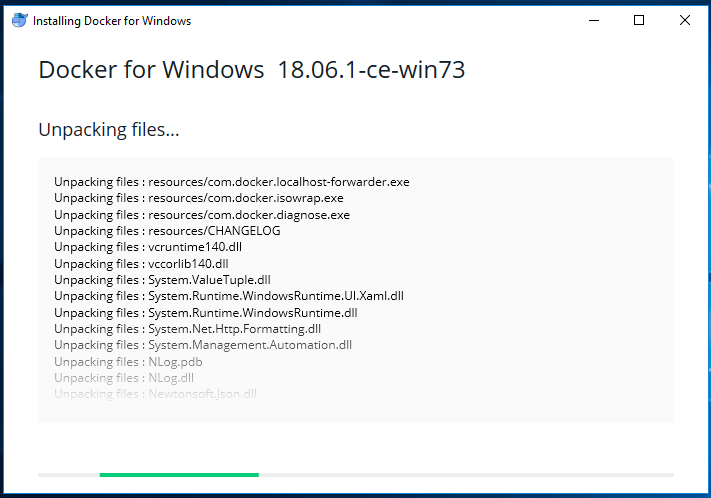
\includegraphics[width=\linewidth]{RE05_Docker/Instalacion_Windows/REDocker_Instalacion_Windows03.png}
	\vspace{-0.2cm}
	\caption{Asistente instalación Docker: Descompresión de paquetes}
	\label{fig:InstalacionDockerWin3}
\end{figure}

\begin{figure}[!hbtp]
	\centering
	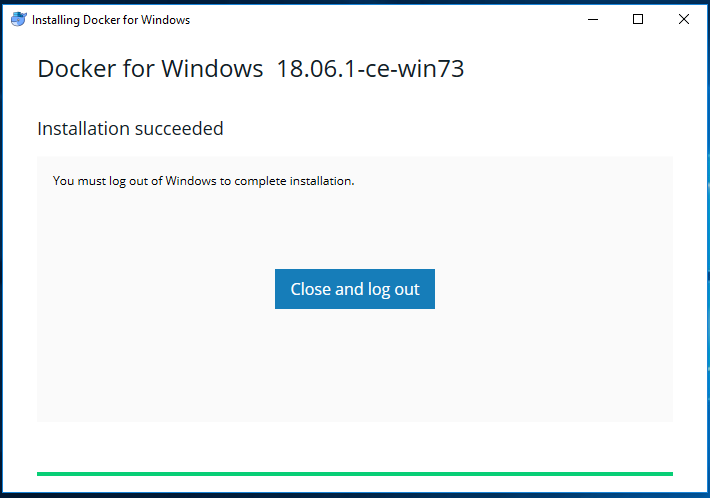
\includegraphics[width=\linewidth]{RE05_Docker/Instalacion_Windows/REDocker_Instalacion_Windows04.png}
	\vspace{-0.2cm}
	\caption{Asistente instalación Docker: Finalización del asistente}
	\label{fig:InstalacionDockerWin4}
\end{figure}

En caso de que se tengan versiones de Microsoft Windows anteriores se puede utilizar Docker Tool Box, herramienta que permite a través de una máquina virtual la gestión de contenedores Docker. Para conocer el proceso de instalación se puede ver el Anexo 2.